
% ----------------------------------------------------------------------
%  Set the document class
% ----------------------------------------------------------------------
\documentclass[11pt,a4paper,twoside]{article}

% ----------------------------------------------------------------------
% Define external packages, language, margins, fonts and new commands
% ----------------------------------------------------------------------
%\input{preamble} 
\usepackage[utf8]{inputenc}   % <<<<< Linux
\usepackage[english]{babel} % <<<<< English
\usepackage{authblk}
\usepackage{notoccite}
\usepackage[skip=0.5\baselineskip]{caption}
\hyphenation{GTKWave}
\usepackage{listings}
\usepackage[all]{nowidow}
\usepackage{float}

%blind text
\usepackage{lipsum}

\usepackage{graphicx}
\graphicspath{ {./} {../../figlib/} }
\def\FontLn{% 16 pt normal
  \usefont{T1}{phv}{m}{n}\fontsize{16pt}{16pt}\selectfont}
\def\FontLb{% 16 pt bold
  \usefont{T1}{phv}{b}{n}\fontsize{16pt}{16pt}\selectfont}
\def\FontMn{% 14 pt normal
  \usefont{T1}{phv}{m}{n}\fontsize{14pt}{14pt}\selectfont}
\def\FontMb{% 14 pt bold
  \usefont{T1}{phv}{b}{n}\fontsize{14pt}{14pt}\selectfont}
\def\FontSn{% 12 pt normal
  \usefont{T1}{phv}{m}{n}\fontsize{12pt}{12pt}\selectfont}

% Use Arial font as default
%
\renewcommand{\rmdefault}{phv}
\renewcommand{\sfdefault}{phv}
\usepackage{geometry}	
\geometry{verbose,tmargin=2.5cm,bmargin=2.5cm,lmargin=2.5cm,rmargin=2.5cm}

%\usepackage{setspace}
%\renewcommand{\baselinestretch}{1.5}

\usepackage[pdftex]{hyperref} % enhance documents that are to be
                              % output as HTML and PDF
\hypersetup{colorlinks,       % color text of links and anchors,
                              % eliminates borders around links
%            linkcolor=red,    % color for normal internal links
            linkcolor=black,  % color for normal internal links
            anchorcolor=black,% color for anchor text
%            citecolor=green,  % color for bibliographical citations
            citecolor=black,  % color for bibliographical citations
%            filecolor=magenta,% color for URLs which open local files
            filecolor=black,  % color for URLs which open local files
%            menucolor=red,    % color for Acrobat menu items
            menucolor=black,  % color for Acrobat menu items
%            pagecolor=red,    % color for links to other pages
            pagecolor=black,  % color for links to other pages
%            urlcolor=cyan,    % color for linked URLs
            urlcolor=black,   % color for linked URLs
	          bookmarks=true,         % create PDF bookmarks
	          bookmarksopen=false,    % don't expand bookmarks
	          bookmarksnumbered=true, % number bookmarks
	          pdftitle={report},
            pdfauthor={Andre C. Marta},
%            pdfsubject={Thesis Title},
%            pdfkeywords={Thesis Keywords},
            pdfstartview=FitV,
            pdfdisplaydoctitle=true}

\usepackage[numbers,sort&compress]{natbib} % <<<<< References in numbered list [1],[2],...
\usepackage{subcaption} 
\usepackage{mdframed}

%%%%%%%%%%%%%%%%%%%%%%%%%%%%%%%%%%%%%%%%%%%%%%%%%%%%%%%%%%%%%%%%%%%%%%%%
%     Begin Document                                                   %
%%%%%%%%%%%%%%%%%%%%%%%%%%%%%%%%%%%%%%%%%%%%%%%%%%%%%%%%%%%%%%%%%%%%%%%%


\begin{document}

% Set plain page style (no headers, footer with centered page number)
\pagestyle{plain}

% Set roman numbering (i,ii,...) before the start of chapters
%\pagenumbering{roman}

% ----------------------------------------------------------------------
%  Cover page
% ----------------------------------------------------------------------
%%%%%%%%%%%%%%%%%%%%%%%%%%%%%%%%%%%%%%%%%%%%%%%%%%%%%%%%%%%%%%%%%%%%%%%%
%                                                                      %
%     File: Thesis_FrontCover.tex                                      %
%     Tex Master: Thesis.tex                                           %
%                                                                      %
%     Author: Andre C. Marta                                           %
%     Last modified :  2 Jul 2015                                      %
%                                                                      %
%%%%%%%%%%%%%%%%%%%%%%%%%%%%%%%%%%%%%%%%%%%%%%%%%%%%%%%%%%%%%%%%%%%%%%%%

\thispagestyle {empty}

% IST Logo - Signature A
% parameters: bb=llx lly urx ury (bounding box), width=h_length, height=v_length, angle=angle, scale=factor, clip=true/false, draft=true/false. 
\includegraphics[bb=9.5cm 11cm 0cm 0cm,scale=0.29]{IST_A_CMYK_POS}

\begin{center}
%
% Figure (Image or plot)
\vspace{1.0cm}
% height = 50 mm
%\includegraphics[height=50mm]{Figures/Airbus_A350.jpg}

% Title, author and degree
\vspace{0.75cm}
{\FontLb T1 - Circuit Analysis Methods} \\ % <<<<< EDIT TITLE
\vspace{0.75cm}
{\FontSn Mestrado Integrado em Engenharia Física Tecnológica} \\ % <<<<< EDIT COURSE
\vspace{0.75cm}
{\FontSn João Lehodey (96538), Jorge Silva (96545), Pedro Monteiro (93156) } \\
\vspace{0.75cm}
{\FontSn March, 2021} \\ % <<<<< EDIT DATE (corresponds to date of oral examination)
%
\end{center}



% ----------------------------------------------------------------------
% Dedication page (optional)
% ----------------------------------------------------------------------
%\input{dedication} 
%\cleardoublepage

% ----------------------------------------------------------------------
%  Acknowledgments (optional)
% ----------------------------------------------------------------------
%\input{acknowledgements}
%\cleardoublepage

% ----------------------------------------------------------------------
%  Abstract (both in English and Portuguese)
% ----------------------------------------------------------------------
%\input{resumo} 
%\cleardoublepage

%\input{abstract} 

% ----------------------------------------------------------------------
%  Table of contents, list of tables, list of figures and nomenclature
% ----------------------------------------------------------------------

% Table of contents
%
\tableofcontents

% List of tables
%\addcontentsline{toc}{section}{\listtablename}
%\listoftables
%\cleardoublepage 

% List of figures
%\addcontentsline{toc}{section}{\listfigurename}
%\listoffigures
%\cleardoublepage 

% Set arabic numbering (1,2,...) after preface
%
%\setcounter{page}{1}
%\pagenumbering{arabic}

% ----------------------------------------------------------------------
%  Body
% ----------------------------------------------------------------------

\section{Introduction}
\label{sec:introduction}

% state the learning objective 
The objective of this laboratory assignment is to study a circuit containing a
sinusoidal voltage source $V_I$ connected to a resistor $R$ and a capacitor $C$
in series. The circuit can be seen if Figure~\ref{fig:rc}.

\lipsum[1-1]

In Section~\ref{sec:analysis}, a theoretical analysis of the circuit is
presented. In Section~\ref{sec:simulation}, the circuit is analysed by
simulation, and the results are compared to the theoretical results obtained in
Section~\ref{sec:analysis}. The conclusions of this study are outlined in
Section~\ref{sec:conclusion}.

\begin{figure}[h] \centering
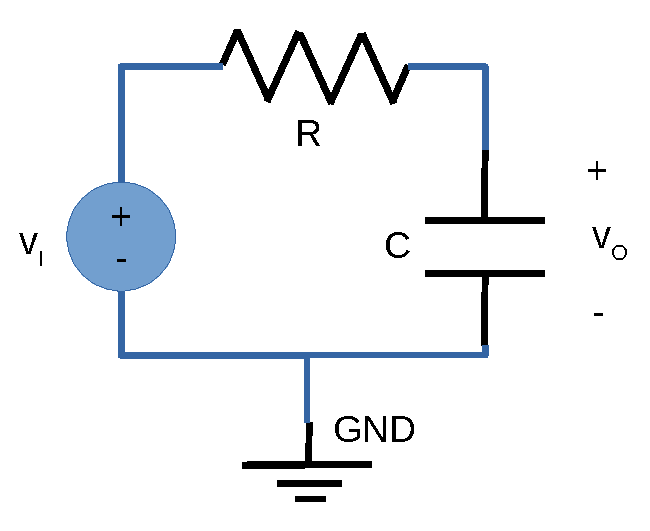
\includegraphics[width=0.4\linewidth]{rc.pdf}
\caption{Voltage driven serial RC circuit.}
\label{fig:rc}
\end{figure}



\section{Theoretical Analysis}
\label{sec:analysis}

In this section, the circuit shown in Figure~\ref{fig:circuit} is analysed
theoretically, first we aproach the circuit using the mesh analysis, and later we analyse the circuit using the nodal analysis.

\subsection{Mesh Analysis}

As seen during theoretical lessons, we can use a mesh analysis to analyse the circuit.
This method is built upon Kirchhoff's Voltage Law that states:

In a mesh, the sum of all voltages equals 0.

\begin{equation}
  \sum_{i=0}^{n} V_i = 0
  \label{eq:kvl}
\end{equation}

The method consists of identifying every mesh, labeling its current, and choosing the direction of the currents.
Then the KVL equations are written for each mesh, and we can solve the system of equations, solving consequently the circuit.

As seen in in Figure~\ref{fig:mesh}, there are four meshes, each with currents $Y_a$, $Y_b$, $Y_c$, $Y_d$, 
we will label each mesh as A, B, C, D respectively.

%image of meshes
\begin{figure}[H] \centering
  \includegraphics[width=0.6\linewidth]{mesh-currents.pdf}
  \caption{Current choosen for each mesh}
  \label{fig:mesh}
\end{figure}

The equations for each mesh are therefore:

% Mesh Equations
\begin{equation*}
  \mathbf{E_1} : y_1 + R_4\cdot(y_1 - y_3) + R_3 \cdot(y_1 - y_2) + y_1 \cdot R_1 = 0
  \label{eq:kvlA}
\end{equation*}
\begin{equation*}
  \mathbf{E_2} : y_2 \cdot (1-R_3 \cdot K_b) + K_b \cdot R_3 \cdot y_1 = 0
  \label{eq:kvlB}
\end{equation*}
\begin{equation*}
  \mathbf{E_3} : y_3 \cdot R_6 + y_3 \cdot R_7 - V_c + (y_3 - y_1) \cdot R_4 = 0
  \label{eq:kvlC}
\end{equation*}
\begin{equation*}
  \mathbf{E_4} : y_4 = I_d
  \label{eq:kvlD}
\end{equation*}
In determining equations $\mathbf{E_1}$ to $\mathbf{E_4}$, we have used the following relations:
\begin{equation*}
  I_b=K_b \times V_b
  \label{eq:extra1}
\end{equation*}
\begin{equation*}
  V_b= R_3 \times (y_2-y_1)
  \label{eq:extra1}
\end{equation*}
\begin{equation*}
  V_c=K_c \times I_c
  \label{eq:extra2}
\end{equation*}
\begin{equation*}
    I_c = y_3
\end{equation*}


In matrix form, the system looks like the following:

\vspace{10mm}

\center{$\begin{bmatrix}
R_1 + R_2 + R_3  &  -R_3                 &  -R_4        &  0 \\
K_{b} R_3        &  1 - R_{3} K_{b}      &  0           &  0 \\
-R_4             & 0                     &  R_{6} + R_7 + R_4 - K_c            &  0 \\
0 & 0 & 0 & 1
\end{bmatrix}$
$\begin{bmatrix}
y_1 \\
y_2 \\
y_3 \\
y_4
\end{bmatrix}$
$=$
$\begin{bmatrix}
  -V_a \\
  0 \\
  0 \\
  I_d
\end{bmatrix}$}

\vspace{20mm}

Solving this system of equations, using the following values generated with the t1\_datagen.py script using the number 93156:


\begin{table}[H]
  \centering
  \begin{tabular}{ c c }
    R1 & 1.03919759193 \\ 
    \hline
    R2 & 2.06836523173 \\ 
    \hline
    R3 & 3.03375774261 \\ 
    \hline
    R4 & 4.12779067183 \\ 
    \hline
    R5 & 3.11985677803 \\ 
    \hline
    R6 & 2.04513887844 \\ 
    \hline
    R7 & 1.04289965713 \\ 
    \hline
    Va & 5.00439410964 \\ 
    \hline
    Id & 1.04536428769 \\ 
    \hline
    Kb & 7.25705461539 \\ 
    \hline
    Kc & 8.23640363075 \\ 
  \end{tabular}
  \caption{Data generated using number 93156}
  \label{tab:data}
\end{table}




We reach the following results, using octave:

 % Table with results created with octave
    \input{../mat/mesh_octave.tex}







%%%%%%%%%% NODAL ANALYSIS

\subsection{Nodal Analysis}

The general point of the node analysis method is to figure out the node voltages of all the nodes in our circuit (in relation to a reference node,
which we call ground, and whose voltage we set to 0). Having figured this out,
it's straightforward to determine the branch currents and voltages, thus completely solving the circuit. 
\par

\begin{figure}[H] \centering
  \includegraphics[width=0.6\linewidth]{nodal.pdf}
  \caption{Nodes used in Nodal Analysis}
  \label{fig:nodal}
\end{figure}

To do this, we first need to identify and label all the nodes in our system as seen in Figure~\ref{fig:nodal},
 as well as choose the ground node. In our case, we defined the node connected to 
 resistance $R_4$ and to voltage source $V_a$ as ground. The second step consists in determining
  the voltages of the easy nodes. In our circuit, it is clear to see, for example, that $e_0 = V_a$.
   To solve the other non-trivial nodes, we proceed to write Kirchhoff's current law for each one of them,
    which states that the sum of currents going into a node must be 0;
     or, in other words, that charges may not accumulate in one singular node:
\begin{equation*}
    \sum_{i} y_i = 0
\end{equation*}
where $y_i$ is a current defined as going \textbf{into} the node.\par
Using Ohm's Law, which states that $I = U/R$, and assuming we know the values of the resistances
 of the elements in each branch (also noticing that we can write the branch
  voltages as differences between node voltages), we get a system of equations that
   allows us to determine each node voltage.
\par
Since this method seems to relies upon Ohm's law, it seems to be a fatal problem that we have a dependent voltage source in our circuit,
$V_c$, for which we \textbf{can't} write ohm's law. To deal with this,
we create a super-node by lumping together the nodes to which $V_c$ is connected and we write KCL
for the super-node. To find the missing equation, we simply note that
$V$(negative terminal of dependent voltage source) + $V_c$ = $V$(positive terminal of dependent voltage source),
thus getting two equations for our two "problematic" nodes.

We can therefore write the following equations:

\begin{equation*}
  \mathbf{Node_1} : e_1 = V_a
  \label{eq:kcl0}
\end{equation*}
\begin{equation*}
  \mathbf{Node_2} : -C_1 \cdot (e_1 - e_2) - C_3 \cdot (e_8 - K_c \cdot C_{6,7} \cdot e_8 - e_2) - C_2 \cdot (e_3 - e_2) = 0
  \label{eq:kcl1}
\end{equation*}
\begin{equation*}
  \mathbf{Node_3} : C_2 \cdot (e_3 - e_2) - K_b \cdot (e_2 - e_8 + K_c \cdot C_{6,7} \cdot e_8) = 0
  \label{eq:kcl2}
\end{equation*}
\begin{equation*}
  \mathbf{Node_6} : C_5 \cdot (e_6 - e_8 + K_c \cdot C_{6,7} \cdot e_8) + K_b \cdot (e_2 - e_8 + K_c \cdot C_{6,7} \cdot e_8) - I_d = 0
  \label{eq:kcl3}
\end{equation*}
\begin{equation*}
    \mathbf{SuperNode} : -C_4 \cdot (-e_8 + K_c \cdot C_{6,7} \cdot e_8) + C_3 \cdot (e_8 - k_c \cdot C_{6,7} \cdot e_8 - e_2) - C_5 (e_6 - e_8 + k_c \cdot C_{6,7} \cdot e_8) + e_8 \cdot C_{6,7} + I_d = 0
\end{equation*}


In determining these equations, we have used, as for the the mesh analysis, the relations:


\begin{equation*}
    I_b = K_b \times V_b
\end{equation*}
\begin{equation*}
    V_b = (e_2 - e_8 + V_c)
\end{equation*}
\begin{equation*}
    V_c = K_c \times I_c
\end{equation*}
\begin{equation*}
    I_c = -e_8 \times C_{6,7}
\end{equation*}

In matrix form, the system of looks like this:
\vspace{10mm}


$\begin{bmatrix}
C_1 + C_2 + C_3  &  -C_2                 &  0        &  -C_3(1-K_c \cdot C_{6,7}) \\
-C_2 - K_b        &  C_2      &  0           &  K_b \cdot (1 - K_c \cdot C_{6,7}) \\
K_b             & 0                     &  C_5
&  -(C_5 + K_b)(1 - K_c C_{6,7}) \\
-C_3 & 0 & -C_5 & (1-K_c \cdot C_{6,7})(C_4 + C_3 + C_5) + C_{6,7}
\end{bmatrix}
\begin{bmatrix}
e_1 \\
e_2 \\
e_3 \\
e_4
\end{bmatrix}
=
\begin{bmatrix}
V_a \cdot C_1 \\
0 \\
I_d \\
-I_d
\end{bmatrix}$

\vspace{10mm}

Solving the system with octave and the previous data we reach the following results:
 % Table with results created with octave
 \input{../mat/nodal_octave.tex}

\section{Simulation Analysis}
\label{sec:simulation}

\subsection{Operating Point Analysis}

\subsubsection{First task}

Table~\ref{tab:op1} shows ---------------------------------

\begin{table}[H]
  \centering
  \begin{tabular}{|l|r|}
    \hline    
    {\bf Name} & {\bf Value [A or V]} \\ \hline
    \input{../sim/op1_tab}
  \end{tabular}
  \caption{Operating point. Variables v(i) are of type {\it voltage} and expressed in
    Volt; other variables are of type {\it current} and expressed in Ampere}
  \label{tab:op1}
\end{table}

The results are the same as the ones obtained using Octave. The subject will be further developed in Section~\ref{sec:conclusion}.

-----------------------------------------------
-----------------------------------------------
-----------------------------------------------
-----------------------------------------------
-----------------------------------------------
-----------------------------------------------
-----------------------------------------------
-----------------------------------------------

\subsubsection{Second task}

Table~\ref{tab:op2} ----------------------------------- 

\begin{table}[H]
  \centering
  \begin{tabular}{|l|r|}
    \hline    
    {\bf Name} & {\bf Value [A or V]} \\ \hline
    \input{../sim/op2_tab}
  \end{tabular}
  \caption{Operating point. Variables v(i) are of type {\it voltage} and expressed in
    Volt; other variables are of type {\it current} and expressed in Ampere}
  \label{tab:op2}
\end{table}

-----------------------------------------------
-----------------------------------------------
-----------------------------------------------
-----------------------------------------------
-----------------------------------------------
-----------------------------------------------
-----------------------------------------------
-----------------------------------------------



\subsubsection{Third task}

Figure~\ref{fig:trans_al3} ----------------------------------- 

\begin{figure}[H] \centering
  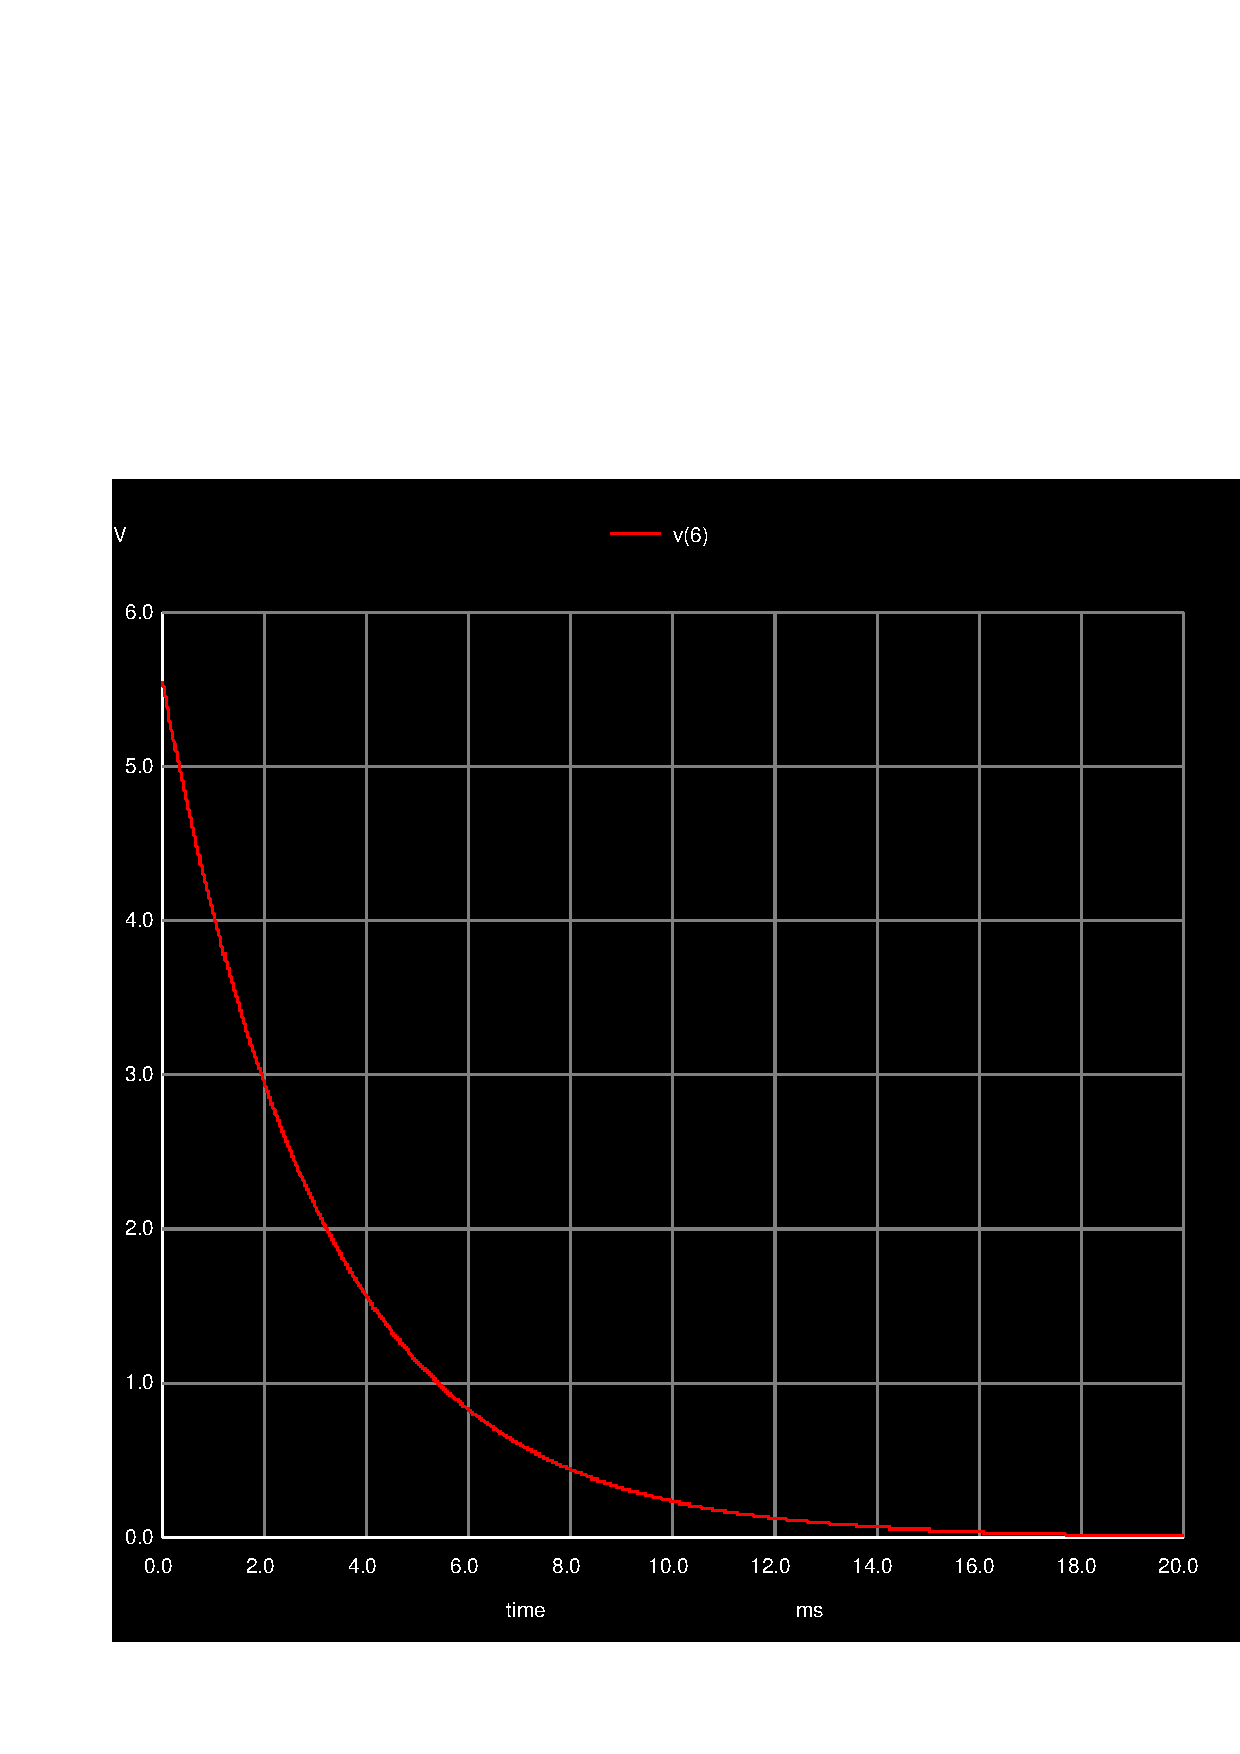
\includegraphics[width=0.6\linewidth]{trans_alinea3.pdf}
  \caption{Transient output voltage of node 6 }
  \label{fig:trans_al3}
  \end{figure}

-----------------------------------------------
-----------------------------------------------
-----------------------------------------------
-----------------------------------------------
-----------------------------------------------
-----------------------------------------------
-----------------------------------------------
-----------------------------------------------


\subsubsection{Fourth task}

Figure~\ref{fig:trans_al4} ----------------------------------- 

\begin{figure}[H] \centering
  \includegraphics[width=0.6\linewidth]{trans_alinea4.pdf}
  \caption{ ---------------------- }
  \label{fig:trans_al3}
  \end{figure}

-----------------------------------------------
-----------------------------------------------
-----------------------------------------------
-----------------------------------------------
-----------------------------------------------
-----------------------------------------------
-----------------------------------------------
-----------------------------------------------



\subsubsection{Fifth task}

Figure~\ref{fig:trans_al5} ----------------------------------- 

\begin{figure}[H] \centering
  \includegraphics[width=0.6\linewidth]{trans_alinea5.pdf}
  \caption{ ---------------------- }
  \label{fig:trans_al3}
  \end{figure}

-----------------------------------------------
-----------------------------------------------
-----------------------------------------------
-----------------------------------------------
-----------------------------------------------
-----------------------------------------------
-----------------------------------------------
-----------------------------------------------


\section{Conclusion}
\label{sec:conclusion}

In this laboratory assignment the objective of analysing an RC circuit has been
achieved. Static, time and frequency analyses have been performed both
theoretically using the Octave maths tool and by circuit simulation using the
Ngspice tool. The simulation results matched the theoretical results
precisely. The reason for this perfect match is the fact that this is a
straightforward circuit containing only linear components, so the theoretical
and simulation models cannot differ. For more complex components, the
theoretical and simulation models could differ but this is not the case in this
work.

\lipsum[1-1]

%\cleardoublepage

% ----------------------------------------------------------------------
%  Bibliography
% ----------------------------------------------------------------------
%\addcontentsline{toc}{section}{\bibname}
%\bibliographystyle{abbrvunsrtnat} % <<<<< SELECT IF USING REFERENCES BY NUMBER (CITATION ORDER)
%\bibliography{../../../BIBfile.bib}

% ----------------------------------------------------------------------
\end{document}
% ----------------------------------------------------------------------

